\section{Защита данных в распределенных системах}
\subsection{Распределенные вычислительные среды}
Распределённая обработка данных - методика выполнения прикладных программ группой систем.
При этом пользователь получает возможность работать с сетевыми службами и прикладными процессами,
расположенными в нескольких взаимосвязанных абонентских системах. \autocite{Sergeeva}

\paragraph{
    Распределенная обработка информации в среде клиент-сервер.
    Концепция распределенной вычислительной среды Distributed Computing Environment (DCE).
    Распределенные базы данных в сетях ЭВМ
} ~\\

Компьютер (или программу), управляющий ресурсом, называют сервером этого ресурса (файлсервер, сервер базы данных,
вычислительный сервер...). Клиент и сервер какого-либо ресурса могут находиться как в рамках одной вычислительной системы,
так и на различных компьютерах, связанных сетью. Основной принцип технологии "клиент-сервер" заключается в разделении
функций приложения на три группы:
\begin{itemize}
    \item ввод и отображение данных (взаимодействие с пользователем);
    \item прикладные функции, характерные для данной предметной области;
    \item функции управления ресурсами (файловой системой, базой данных и т.д.)
\end{itemize}

Поэтому, в любом приложении можно выделить следующие компоненты:
\begin{itemize}
    \item компонент представления данных
    \item прикладной компонент
    \item компонент управления ресурсом
\end{itemize}

Связь между компонентами осуществляется по определенным правилам, которые называют "протокол взаимодействия".
Каждый из компонентов приложения при этом может работать на выделенном сервере (узле) или разделять ресурсы сервера
с другими компонентами приложения. В связи с этим можно выделить следующие модели приложений:
\begin{itemize}
    \item двухзвенная модель (модель «клиент-сервер»)
    \item трехзвенная модель (модель сервера приложений)
    \item многозвенная модель
\end{itemize}

\textbf{Двухзвенная модель} позволяет распределить различным образом три компонента приложения между двумя узлами.
\textbf{Трехзвенная модель} предполагает выделение для каждого из трех компонентов приложения свой сервер.
\textbf{Многозвенная модель} позволяет отдельным компонентам использовать ресурсы нескольких серверов, например,
распределенные базы данных. Компанией Gartner Group, специализирующейся в области исследования информационных технологий,
предложена следующая классификация двухзвенных моделей взаимодействия клиент-сервер \autocite{dce}
\begin{figure}[h!]
    \centering
    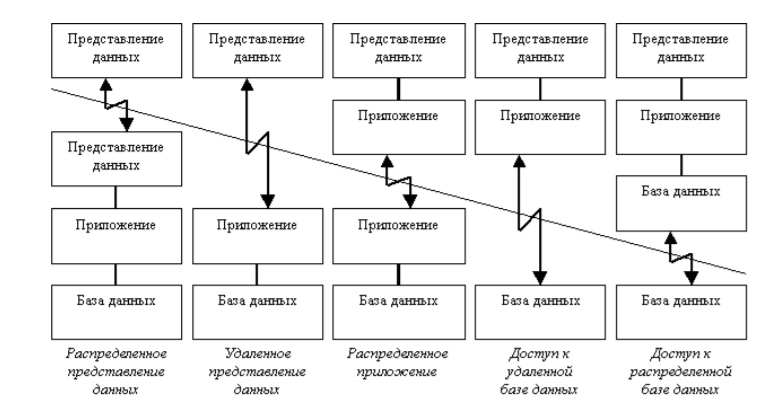
\includegraphics[width=0.8\textwidth]{assets/dce.jpg}
    \caption{Классификация двухзвенных моделей}
\end{figure}

Появление сетей ЭВМ позволило наряду с централизованными создавать и распределенные базы данных.
\textbf{Распределенная база данных} состоит из нескольких, возможно, пересекающихся или да­же дублирующих друг друга
частей, хранимых в различных ЭВМ вычислительной сети. Однако пользователь распределенной базы данных не обязан
знать, каким образом ее компоненты размещены в узлах сети, и представляет себе эту базу данных как единое
це­лое. Работа с такой базой данных осуществляется с помощью \textit{сис­темы управления распределенной базой данных} (СУРБД).
\\

\subsection{Угрозы безопасности распределенных СУБД}
\paragraph{Угрозы доступности, целостности и конфиденциальности данных. Механизмы противодействия} ~\\

\textbf{Современный подход к информационной безопасности}

Под информационной безопасностью понимается защита информации и поддерживающей ее инфраструктуры с помощью
совокупности программных, аппаратно-программных средств и методов, а также организационных мер, с целью недопущения
причинения вреда владельцам этой информации или поддерживающей ее инфраструктуре.

При построении системы защиты должен учитываться комплексный подход в обеспечении безопасности информации.
Он подразумевает использование защитных механизмов на всех этапах жизненного цикла системы, от ее проектирования
и до вывода из эксплуатации, и совместное решение целого спектра вопросов, начиная от физической защиты объектов ИС,
с применением интеллектуальной системы контроля доступа, и заканчивая вопросами поддержки нормального функционирования
ИС в критических ситуациях.

Проектирование системы безопасности информации (СБИ) осуществляется совместно с проектированием самой информационной системы.
При внесении любых изменений в структуру ИС, это должно найти адекватное отражение и в системе защиты.

При разработке систем информационной безопасности необходимо учитывать передовые тенденции развития информационных
технологий, к каким в настоящее момент относятся интрасети (Интранет - Intranet).
Характерными чертами данных сетей является то, что они основываются на технологии клиент/сервер, имеют в своем составе
разнородные корпоративные информационные системы и пользуются внешними сервисами, базовым для которых является
протокол TCP/IP, а также предоставляет аналогичные сервисы вовне. Центральным элементом интрасетей является
WEB-сервис, поэтому чрезвычайно важным является вопрос обеспечения защищенности этого сервиса.

\bigbreak
\textbf{Разработка политики безопасности}

Первым шагом на пути построения СБИ является разработка политики безопасности ИС.
Под политикой безопасности следует понимать утвержденный высшим должностным лицом организации, в
интересах которой разрабатывается ИС и система защиты, документ, с указанием организационных и технических мероприятий,
направленных на защиту информации, и поддерживающей ее инфраструктуры.

В данном документе должны найти обязательное отражение основные принципы безопасности информации,
такие как многоуровневая защита и разнообразие средств и методов защиты, минимизация привилегий, разделение полномочий,
невозможность обхода средств защиты и т.п.

\bigbreak
\textbf{Построение модели нарушителя}

После разработки политики безопасности производится анализ угроз ИС, возможных каналов утечки информации и
построение на этой основе модели потенциального нарушителя.

Согласно предлагаемой модели, в качестве нарушителя может выступать как отдельное физическое лицо,
так и специальные программы, содержащие в себе некие деструктивные элементы - разрушающие программные компоненты (РПК).

Под объектом защиты в данной модели понимается материальный носитель защищаемой информации, а также сама информация,
доступ к которым определен режимом разграничения доступа, реализуемым системой защиты, а также поддерживающая инфраструктура.

Предполагается, что по отношению к ИС нарушитель может быть двух типов: внутренним или внешним.
При этом внутренний нарушитель выступает в качестве законного пользователя системы или лица из числа
обслуживающего персонала или администрации ИС, а внешний является лицом, не подпадающим ни под
одну из указанных категорий. РПК, в свою очередь, может быть отнесено к категории внутреннего нарушителя.

Возможные угрозы нарушителя напрямую зависят от его типа. Возможности внутреннего нарушителя ограничены
установленными правилами разграничения доступа, внутриобъектовым режимом и его функциональными обязанностями.
Возможности РПК в ИС намного шире и определяются работоспособностью ПО, в котором они заложены,
а также наличием в системе средств активного аудита и мониторинга.

\bigbreak
\textbf{Проектирование СБИ}

Следующим шагом после разработки модели нарушителя является проектирование СБИ.
Согласно принципу многоуровневой защиты и разнообразия средств и методов защиты, можно выделить следующие
самостоятельные системы в составе СБИ (при этом необходимо учитывать, что все они интегрированы
и находятся в тесной взаимосвязи):
\begin{itemize}
    \item Система контроля доступа на объекты и в помещения ИС
    \item Система защиты информации в ИС от НСД
    \item Средства защиты от РПК
    \item Средства поддержания доступности информации в ИС
\end{itemize}

\bigbreak
\textbf{Система защиты информации в ИС от НСД}

Данная система может быть реализована как встроенными средствами защиты сетевых операционных
систем и систем управления базами данных (СУБД), так и дополнительными средствами. Стоит лишь отметить,
что при построении системы защиты от НСД необходимо, по возможности, избегать дублирования многих функций,
с тем, чтобы СБИ не страдала избыточностью, что в конечном итоге скажется как на удобстве работы
пользователей и их желании выполнять все предписания системы защиты, так и на управляемости самой СБИ.

В состав указанной системы также должны входить:
\begin{itemize}
    \item средства контроля, управления и идентификации при удаленном доступе
    \item средства управления доступом и идентификации в рамках ИС
    \item средства экранирования ИС от открытых сетей, а также разноуровневых сетей внутри данной ИС друг от друга
    \item средства управления, анализа и аудита СБИ в рамках сетевых конфигураций
\end{itemize}

\bigbreak
\textbf{Средства контроля, управления и идентификации при удаленном доступе к ИС}

Указанная категория средств предназначена для осуществления процедуры контроля подключения к ИС удаленных пользователей,
а также для управления их доступом и осуществления идентификации. Данная проблема возникает в связи со структурой
интрасетей, когда удаленные пользователи получают доступ к ресурсам корпоративной ИС по выделенным,
либо коммутируемым каналам связи. В этом случае существует реальная вероятность несанкционированного подключения
нарушителя к линии связи, с активным или пассивным прослушиванием сети и выдачей себя за
регистрированного пользователя ИС. В целях недопущения подобного целесообразно применение методов с
использованием одноразовых паролей и единого входа в сеть

Принцип систем с одноразовыми паролями основан на однократном использовании пароля для процедуры
идентификации в ИС, в результате чего перехват его нарушителем становится бессмысленным.
Идентификация и аутентификация пользователя осуществляется сервером безопасности (аутентификации), входящим в состав ИС.

Концепция единого входа в сеть предоставляет существенное удобство для пользователей, так как при
подключении к ИС им достаточно только один раз доказать свою подлинность. Кроме этого, применение
этой концепции способствует усилению информационной безопасности, ввиду того, что в сети
отсутствует открытая передача аутентификационной информации.

\bigbreak
\textbf{Средства управления доступом и идентификации в рамках ИС}

Учитывая территориальную разнесенность современных ИС и использование технологии клиент/сервер,
целесообразно выделение функции проверки подлинности в виде отдельного сервера безопасности (аутентификации).
Услугами данного сервера должны пользоваться все другие серверы и пользователи ИС.

Сервер безопасности может быть реализован в виде одного или нескольких серверов, функционирующих на физически
защищенных компьютерах. Серверы должны содержать репозиторий субъектов ИС и их секретные ключи.

При построении сервера безопасности возможны два пути:
\begin{itemize}
    \item Сервер безопасности с центральным хранением данных репозитория
    \item Сервер безопасности с децентрализованным хранением данных репозитория
\end{itemize}

Однако централизованное хранение является нецелесообразным по следующим причинам:
\begin{itemize}
    \item сильная зависимость от готовности сервера
    \item возможность расширения или комбинирования сетей в процессе развития ИС
\end{itemize}

Дополнительной причиной децентрализации сервера безопасности является объединение сетей при развитии ИС.
Возможна ситуация, когда две до того независимые сети, имеющие каждая в своем составе отдельный сервер безопасности,
объединяются. В этом случае один из серверов должен быть уничтожен, а все определенные в нем данные по авторизации
переданы на другой сервер. Если же связь между двумя сетями устанавливается временно, то необходимо наличие
нескольких серверов безопасности. В противном случае, один сервер должен будет производить постоянные,
двойные определения то для одной, то для другой сети. Для того, чтобы избежать этого, необходимо
наличие нескольких серверов безопасности.

\bigbreak
\textbf{Средства экранирования ИС}

Средства экранирования используются для подключения ИС к открытым сетям или развязки разноуровневых сетей,
т.е. сетей, обрабатывающих информацию с различным грифом секретности. Концепция систем типа Firewall
(брандмауер, межсетевой экран) была разработана для снижения риска нелегального доступа к закрытой информации при
подключении частных сетей (в том числе ЛВС) к сетям общего пользования. Межсетевой экран представляет собой
программно-аппаратный комплекс, размещенный на стыке двух сетей и реализующий следующие три функции:
\begin{itemize}
    \item обеспечение обмена данными между сетями только через указанную систему
    \item фильтрация трафика обмена
    \item предотвращение возможности проникновения в сам экран
\end{itemize}

В этом случае обеспечивается эффективная блокировка внешнего трафика частной сети и жесткий контроль за ним.
Кроме того экраны могут осуществлять разграничение доступа между различными сегментами одной корпоративной сети,
а также контроль за информационными потоками, направленными во вне, обеспечивая тем самым необходимый
режим конфиденциальности.

Применение экранов также позволяет существенно уменьшить уязвимость внутренних сервисов безопасности, так
как нарушителю необходимо вначале преодолеть защитные механизмы самого экрана,
где они сконфигурированы особенно тщательно.

Существующие в настоящее время экраны могут быть условно разделены на следующие четыре типа:
\begin{itemize}
    \item экраны с фильтрацией пакетов (packet-filtering firewall)
    \item шлюзы сеансового уровня (circuit-level gateway)
    \item шлюзы прикладного уровня (application-level gateway)
    \item экраны экспертного уровня (stateful inspection firewall)
\end{itemize}

Однако лишь некоторые экраны могут быть отнесены только к одной из указанный категорий.
При этом необходимо отметить, что экраны экспертного уровня обеспечивают один из самых высоких на сегодняшний
день уровней безопасности интрасетей.

\bigbreak
\textbf{Средства управления, анализа и аудита}

Средства аудита занимают свое особое положение в ряду средств обеспечения безопасности информации,
заключающееся в том, что все действия нарушителя по преодолению средств защиты фиксируются, позволяя тем самым
вовремя обнаружить попытку несанкционированного входа в ИС. Причем, учитывая принцип многоуровневой защиты,
нарушителю придется преодолевать несколько защитных рубежей, что будет обязательно отмечено в регистрационном
протоколе. В случае если указанная процедура выполняется в режиме реального времени, администратором безопасности
могут быть своевременно предприняты соответствующие меры по предотвращению незаконного вторжения на одном из
следующих уровнях защиты.

Кроме средств аудита часть программных продуктов также позволяет осуществлять оценку системы безопасности сети,
имитируя все известные способы, применяемые нарушителями для проникновения в интрасети, и тем самым, обнаруживая
в системе защиты слабые места. Данные программные продукты не только выявляют уязвимые места, но и определяют
действия, которые необходимо предпринять для ликвидации пробелов в сетевой системе безопасности. Администратору
остается лишь выбрать способы их устранения.

\bigbreak
\textbf{Средства резервного копирования}

Резервное копирование программ и данных необходимо проводить с целью минимизации потерь в случае отказов
оборудования, либо сбоев в программном обеспечении ИС. Данная задача наиболее сложна именно в интрасетях
с их распределенными ресурсами и неоднородностью, в которых работают компьютеры под управлением различных
операционных систем. Учитывая клиент/серверный характер интрасетей функцию резервного копирования целесообразно
также выделить в виде отдельного сервера (сервера архива).

Распространение клиент/серверного подхода на процедуру резервного копирования информации и данных
имеет ряд преимуществ по сравнению с традиционными методами. Они выражаются в следующем:
\begin{itemize}
    \item Администраторы рабочих групп освобождаются от необходимости согласования действий
    и самой процедуры создания локальных резервных копий
    \item Единообразие процедуры создания резервных копий в ИС
    \item Возможность мониторинга процесса резервирования и диагностики возникших проблем
\end{itemize}

Одним из способов обеспечения высокой доступности информации является создание резервных копий с возможностью
ее хранения в двух местах: один экземпляр хранится поблизости от оригинала, а другой в удаленном безопасном месте.

\bigbreak
\textbf{Безопасность систем управления базами данных}

Составной частью информационной безопасности ИС является безопасность систем управления
базами данных (СУБД). Учитывая, что СУБД является ключевым элементом современной ИС, можно отметить, что
для них важны все три аспекта информационной безопасности: конфиденциальность, целостность и доступность.

В СУБД для идентификации и проверки подлинности применяются либо соответствующие механизмы операционной
системы, либо специальный SQL-оператор.

\bigbreak
\textbf{Обеспечение конфиденциальности данных}

В СУБД, как правило, используется произвольное управление доступом, когда владелец объекта передает
права доступа к нему (привилегии) по своему усмотрению. При этом привилегии в СУБД можно подразделить на две
категории: привилегии безопасности и привилегии доступа.

Привилегии безопасности всегда выделяются конкретному пользователю и позволяют выполнять административные действия.

Привилегии доступа определяют права доступа субъектов к определенным объектам.

Специфическим механизмом управления доступом в СУБД являются представления. Они позволяют сделать
видимыми для субъектов только те столбцы базовых таблиц, доступ к которым предоставлен субъектам администратором базы.

\bigbreak
\textbf{Поддержание целостности}

Целостность данных не менее важна, чем конфиденциальность, ввиду того, что для баз данных, как и для
ИС в целом, главными врагами являются не внешние нарушители, а ошибки оборудования, программ, администраторов и
пользователей системы.

С точки зрения пользователей СУБД, основными средствами поддержания целостности данных являются ограничения и правила.

Ограничения могут относиться как к таблицам, так и к отдельным столбцам. Они накладываются владельцами
таблицы и оказывают влияние на все операции с данными.

Правила позволяют вызывать выполнение заданных действий при определенных изменениях базы данных.
В отличие от ограничений, являющихся лишь средствами контроля простых условий, правила позволяют
создавать сколь угодно сложные соотношения между различными элементами базы данных.

\bigbreak
\textbf{Обеспечение доступности данных}

Доступность данных подразумевает обеспечение информационной системы средствами поддержания высокой
доступности. Поддержание высокой доступности позволяет свести к минимуму возможные сбои аппаратного
обеспечения, в частности носителей информации, а также ошибки обслуживающего персонала и программного
обеспечения. В качестве мер поддержания высокой доступности может быть названа кластеризация сервера баз
данных (выделение нескольких компьютеров, выполняющих общее приложение), а также тиражирование данных
(хранение базы данных в различных местах).

\bigbreak
\textbf{Угрозы СУБД}

СУБД отличаются от других компонентов ИС специфичными угрозами, и главным их источником является
сама природа баз данных. Известно, что основным средство общения с СУБД выступает язык SQL,
являющийся мощным инструментом манипулирования данными. С его помощью, используя механизм правил, могут
быть созданы сложные, трудно поддающиеся анализу цепочки действий, позволяющие не явным образом передавать
право на выполнение определенных процедур тем, кто не имеет на это полномочий.

В качестве примера можно привести несколько угроз, возникающих при использовании языка SQL: получение
информации путем логических выводов, агрегирование данных, покушение на высокую доступность.

Методы борьбы против получения информации путем логических выводов состоят в тщательном проектировании
модели данных, иерархии привилегий и видимых пользователям представлений.

Агрегирование данных состоит в получении новой информации путем комбинирования данных, полученным официальным
путем. Причем информация, содержащаяся в скомбинированных данных, может иметь гриф более высокий, чем первичная информация.

Методом борьбы с агрегированием может быть тщательное проектирование модели данных и максимально допустимое
ограничение доступа пользователей к информации.

Покушение на высокую доступность может быть реализовано, если пользователю-нарушителю доступны все возможности
языка SQL. При этом он легко сможет заблокировать работу других пользователей. Поэтому, в целях борьбы с данным
видом угроз, рекомендуется запрещать непосредственный SQL-доступ к базе данных, используя для этого серверы приложений.


\subsection{Распределенная обработка данных}
\paragraph{Понятие распределенной транзакции}~\\
Если данные хранятся в одной базе данных, то транзакция к ней рассматривается как локальная.
В распределенных базах транзакция, выполнение которой заключается в обновлении данных на нескольких узлах сети,
называется глобальной или \textbf{распределенной транзакцией}.

Внешне выполнение распределенной транзакции выглядит как обработка транзакции к локальной базе данных.
Тем не менее распределенная транзакция включает в себя несколько локальных транзакций, каждая из которых
завершается двумя путями — фиксируется или прерывается. Распределенная транзакция фиксируется только в том случае,
когда зафиксированы все локальные транзакции, ее составляющие.

\paragraph{Модель обработки транзакций} ~\\
В стандарте ANSI/ISO SQL определены модель транзакций и функции операторов COMMIT и ROLLBACK.
Стандарт определяет, что транзакция начинается с первого SQL-оператора, инициируемого пользователем или содержащегося
в программе. Все последующие SQL-операторы составляют тело транзакции. Транзакция завершается одним из четырех
возможных путей:
\begin{itemize}
    \item оператор COMMIT означает успешное завершение транзакции; его использование делает постоянными изменения,
    внесенные в базу данных в рамках текущей транзакции
    \item оператор ROLLBACK прерывает транзакцию, отменяя изменения, сделанные в базе данных в рамках
    этой транзакции; новая транзакция начинается непосредственно после использования ROLLBACK
    \item успешное завершение программы, в которой была инициирована текущая транзакция,
    означает успешное завершение транзакции (как будто был использован оператор COMMIT)
    \item ошибочное завершение программы прерывает транзакцию (как будто был использован оператор ROLLBACK)
\end{itemize}

Точки сохранения применяются, как правило, в протяженных транзакциях и позволяют разделить транзакцию на несколько
небольших осмысленных фрагментов. Пользователь может зафиксировать работу в любой точке транзакции с тем,
чтобы выполнить ее откат к состоянию, соответствующему этой точке.

Откат и фиксация транзакций становятся возможными благодаря журналу транзакций. Он используется следующим образом.
Известно, что все операции над реляционной базой данных суть операции над строками таблиц. Следовательно,
для обеспечения отката таблиц к предыдущим состояниям достаточно хранить не состояния таблицы, а лишь те
ее строки, которые подверглись изменениям.

При выполнении любого оператора SQL, который вносит изменения в базу данных, СУБД автоматически заносит
очередную запись в журнал транзакций. Запись состоит из двух компонентов: первый - это состояние строки до
внесения изменений, второй - ее же состояние после внесения изменений. Только после записи в журнал транзакций
СУБД действительно вносит изменения в базу данных. Если после данного оператора SQL был выполнен оператор
COMMIT, то в журнале транзакций делается отметка о завершении текущей транзакции. Если же после
оператора SQL следовал оператор ROLLBACK, то СУБД просматривает журнал транзакций и отыскивает записи,
отражающие состояние измененных строк до внесения изменений. Используя их, СУБД восстанавливает те
строки в таблицах базы данных, которые были изменены текущей транзакцией, - таким образом
аннулируются все изменения в базе данных.

\paragraph{Мониторы обработки транзакций}~\\
Мониторы обработки транзакций (Transaction Processing Monitor - TPM), или, проще, мониторы
транзакций - программные системы (которые относят к категории middleware, то есть к посредническому
или промежуточному программному обеспечению), обеспечивающие эффективное управление информационно-вычислительными
ресурсами в распределенной системе. Они представляют собой гибкую, открытую среду для разработки и
управления мобильными приложениями, ориентированными на оперативную обработку распределенных транзакций.
В числе важнейших характеристик TPM - масштабируемость, поддержка функциональной полноты и целостности
приложений, достижение максимальной производительности обработки данных при невысоких стоимостных
показателях, поддержка целостности данных в гетерогенной среде. TPM опираются на трехзвенную
модель "клиент-сервер" (модель сервера приложений или AS-модель), описанную в Разделе 2.
Естественно, что все преимущества модели отражаются и на программных системах, построенных на ее основе.

На современном рынке мониторов транзакций основными "действующими лицами" являются такие системы,
как ACMS (DEC), CICS (IBM), TOP END (NCR), PATHWAY (Tandem), ENCINA (Transarc), TUXEDO System (USL).
Несмотря на принципиальное сходство, конкретные TPM отличаются рядом характеристик, причем
различия часто вытекают как из специфики операционной системы, в которой реализован и функционирует TPM.

\paragraph{Корпоративная среда обработки транзакций}~\\

TPM на базе UNIX опирается на фундаментальное понятие - корпоративную среду обработки транзакций
(Enterprise Transaction Processing - ETP). Архитектура ETP - это три ряда компьютеров:
\begin{itemize}
    \item Ряд 1: Персональные станции (Personal Workstations);
    \item Ряд 2: Компьютеры под управлением ОС UNIX (UNIX Transaction Processing Servers - UPTS);
    \item Ряд 3: Mainframe-системы (Proprietary Transaction Processing Servers - PTPS)
    или компьютеры под управлением UNIX c RISC-архитектурой процессоров;
\end{itemize}

Компьютеры \textbf{ряда 1}, функционирующие под управлением DOS, MS Windows, OS/2, UNIX, используются в качестве рабочих мест
конечных пользователей. Характерная черта ETP - отсутствие ограничений на модели компьютеров,
составляющих этот ряд. Однако, как правило, ряд 1 состоит из компьютеров на базе процессоров Intel
486/Pentium под управлением MS Windows (MS Windows фактически стала стандартом оконного графического интерфейса
для большинства категорий пользователей и стандартом операционной среды для подавляющего числа прикладных программ и систем).

\textbf{Ряд 2} составляют компьютеры среднего класса под управлением ОС UNIX,
на которых функционирует ядро TPM и, как правило, реляционные СУБД (Oracle, Informix, Ingres),
выступающие в качестве менеджера ресурсов. Кроме того, на них же может быть установлен шлюз к TPM в
операционной среде мэйнфрейма (как правило, разработчики TPM на базе UNIX предусматривают в конфигурации своих
систем шлюз к наиболее популярной такой системе - IBM CICS).

\textbf{Ряд 3} представлен мэйнфреймами или RISC-компьютерами под управлением UNIX. О мэйнфреймах мы
говорим в тех ситуациях, когда исторически сложилось так, что в организации они существуют уже долгое время,
берут на себя большую часть всего объема обработки транзакций, концетрируют огромные вычислительные
ресурсы и содержат большие массивы данных (то есть речь идет об унаследованных системах). Если этого
"тяжелого наследия" нет, то можно смело использовать в качестве компьютеров ряда 3 RISC-серверы,
сегодня приближающиеся по производительности к мэйнфреймам.

Таким образом, среда обработки транзакций формируется из набора разнородных компьютеров (и соответствующих ОС),
ранжируемых от персональных компьютеров до мэйнфрейм-систем. TPM на базе UNIX представляет собой своего
рода "клей", который связывает вместе компьютеры трех рядов в открытую унифицированную среду обработки транзакций.

Ключом к интеграции систем, функционирующих на компьютерах различных рядов, является специализированный
интерфейс прикладного программирования ATMI (Application Transaction Manager Interface), обеспечивающий:
\begin{itemize}
    \item для ряда 1 - формирование и передачу запросов от клиентов к серверам, выполняющимся на компьютерах ряда 2
    \item для ряда 2 - обработку запросов, поступающих от компьютера ряда 1 (в том числе и с
    обращением к менеджеру ресурсов), и, по необходимости, формирование и направление
    запросов к серверам, выполняющимся на компьютерах ряда 3
    \item для ряда 3 - обработку запросов, поступающих от серверов ряда 2
\end{itemize}

Стоит отметить, что подобное представление о корпоративной среде обработки транзакций не является абстракцией.
Сегодня многие организации приходят именно к такой, "трехуровневой"  архитектуре информационных
систем (с той оговоркой, что наличие ряда 3 вызвано историческими причинами - мэйнфреймы использовались
первоначально и сразу от них отказаться невозможно).

\subsection{Протоколы фиксации}
\paragraph{Протоколы фиксации}~\\

В локальной системе базы данных для принятия транзакции диспетчер транзакций должен только передать решение
о фиксации диспетчеру восстановления. Однако в распределенной системе диспетчер транзакций должен передать
решение о фиксации всем серверам в различных сайтах, где выполняется транзакция, и обеспечить
единообразное выполнение решения. Когда обработка завершается на каждом сайте, она достигает состояния
частично подтвержденной транзакции и ожидает, пока все другие транзакции достигнут их частично подтвержденных состояний.
Когда он получает сообщение о том, что все сайты готовы к фиксации, он начинает фиксировать.
В распределенной системе либо все сайты фиксируют, либо ни один из них не делает.

Различные протоколы распределенной фиксации:
\begin{itemize}
    \item Однофазный коммит
    \item Двухфазный коммит
    \item Трехфазный коммит
\end{itemize}

\bigbreak
\textbf{Распределенная однофазная фиксация}

Распределенная однофазная фиксация – это самый простой протокол фиксации. Давайте рассмотрим, что есть
контролирующий сайт и несколько подчиненных сайтов, где выполняется транзакция. Шаги в распределенном коммите:
\begin{itemize}
    \item После того, как каждое ведомое устройство локально завершило свою транзакцию, оно
    отправляет сообщение «ГОТОВО» на контролирующий сайт
    \item Подчиненные ожидают сообщения «Подтвердить» или «Прервать» с контролирующего сайта.
    Это время ожидания называется окном уязвимости
    \item Когда контролирующий сайт получает сообщение «СДЕЛАНО» от каждого ведомого, он принимает решение
    о фиксации или отмене. Это называется точкой фиксации. Затем он отправляет это сообщение всем рабам
    \item При получении этого сообщения ведомое устройство либо фиксирует, либо прерывает работу,
    а затем отправляет подтверждающее сообщение на контролирующий сайт
\end{itemize}

После того, как каждое ведомое устройство локально завершило свою транзакцию, оно отправляет сообщение
«ГОТОВО» на контролирующий сайт.

Подчиненные ожидают сообщения «Подтвердить» или «Прервать» с контролирующего сайта. Это время ожидания
называется окном уязвимости.

Когда контролирующий сайт получает сообщение «СДЕЛАНО» от каждого ведомого, он принимает решение о
фиксации или отмене. Это называется точкой фиксации. Затем он отправляет это сообщение всем рабам.

При получении этого сообщения ведомое устройство либо фиксирует, либо прерывает работу,
а затем отправляет подтверждающее сообщение на контролирующий сайт.

\bigbreak
\textbf{Распределенная двухфазная фиксация}
Распределенная двухфазная фиксация снижает уязвимость однофазных протоколов фиксации. Шаги, выполняемые на двух этапах:
\bigbreak
\textbf{Этап 1}
\begin{itemize}
    \item После того, как каждое ведомое устройство локально завершило свою транзакцию,
    оно отправляет сообщение «ГОТОВО» на контролирующий сайт. Когда контролирующий сайт получил сообщение «ГОТОВО»
    от всех подчиненных, он отправляет сообщение «Подготовить» подчиненным
    \item Рабы голосуют за то, хотят ли они по-прежнему совершать или нет. Если ведомый
    хочет зафиксировать, он отправляет сообщение «Готово»
    \item Раб, который не хочет коммитить, отправляет сообщение «Не готов». Это может произойти,
    если ведомое устройство имеет конфликтующие параллельные транзакции или истекло время ожидания
\end{itemize}

После того, как каждое ведомое устройство локально завершило свою транзакцию, оно отправляет
сообщение «ГОТОВО» на контролирующий сайт. Когда контролирующий сайт получил сообщение «ГОТОВО» от всех подчиненных,
он отправляет сообщение «Подготовить» подчиненным.

Рабы голосуют за то, хотят ли они по-прежнему совершать или нет. Если ведомый хочет зафиксировать,
он отправляет сообщение «Готово».

Раб, который не хочет коммитить, отправляет сообщение «Не готов». Это может произойти, если ведомое
устройство имеет конфликтующие параллельные транзакции или истекло время ожидания.

\textbf{Этап 2}

\begin{itemize}
    \item После того, как контролирующий сайт получил сообщение «Готово» от всех ведомых –
    \begin{itemize}
        \item Контролирующий сайт отправляет сообщение «Global Commit» подчиненным
        \item Подчиненные устройства применяют транзакцию и отправляют сообщение «Подтвердить ACK» на контролирующий сайт
        \item Когда контролирующий сайт получает сообщение «Подтвердить ACK» от всех ведомых
        устройств, он считает транзакцию подтвержденной
    \end{itemize}
    \item После того, как контролирующий сайт получил первое сообщение «Не готов» от любого ведомого –
    \begin{itemize}
        \item Контролирующий сайт отправляет сообщение «Global Abort» подчиненным
        \item Слэйвы отменяют транзакцию и отправляют сообщение «Abort ACK» на контролирующий сайт
        \item Когда контролирующий сайт получает сообщение «Abort ACK» от всех ведомых
        устройств, он считает транзакцию отмененной
    \end{itemize}

\end{itemize}

\bigbreak
\textbf{Распределенная трехфазная фиксация}
Шаги в распределенной трехфазной фиксации следующие:
\begin{itemize}
    \item Этап 1: Шаги такие же, как при распределенной двухфазной фиксации
    \item Этап 2: Подготовьтесь к фиксации
    \begin{itemize}
        \item Контролирующий сайт выдает широковещательное сообщение «Ввод подготовленного состояния»
        \item Ведомые сайты голосуют «ОК» в ответ
    \end{itemize}
    \item Фиксация / Отмена
\end{itemize}

Этапы аналогичны двухфазной фиксации, за исключением того, что сообщение «Подтвердить ACK» / «Прервать ACK» не требуется

\paragraph{Защищенные протоколы фиксации}
\paragraph{Обработка распределенных транзакций в базах данных с многоуровневой секретностью (MLS)}~\\
Известно, что в MLS/DBMS не ко всем данным, содержащимся в  базе
данных, доступ осуществляется одинаково. Однако современные СУБД, как
правило,  не имеют адекватных средств диагностики и механизма определения
того, что пользователь имеет возможность доступа только  к  тем
данным,  которые являются релевантными. Таким образом, MLS/DBMS отличается
от соответствующих DBMS,  по крайней  мере,  следующими  двумя
особенностями:
\begin{itemize}
    \item каждый элемент данных в базе данных связан с уровнем доступа
    \item доступ пользователя к данным должен контролироваться релевантностью для данного пользователя
\end{itemize}
Разработка сервиса MLS/DBMS в современных компьютерных  системах
представляет  много  проблем. До настоящего времени внедрение многоуровневого
разграничения доступа в операционную  систему  представляет
собой  значительные трудности. Решение этой проблемы в виде аббревиатуры
обозначается ТСВ. Хотя в разрешении вопросов ТСВ  для  удаленных
пользователей  в  MLS/DBMS вводятся компромиссы, остается много проблем,
которые требуется разрешать. Наиболее очевидная проблема состоит
в том, что вопросы классификации в СУБД значительно  сложнее,  чем  в
файловых  системах  и могут быть сложнее реализованы. Другая проблема
состоит в том, что для классификации данных,  содержащих  контекстные
представления,  временные параметры, их композицию, необходимы унифицированные базы данных.

\subsection{Тиражирование данных}
\textbf{Тиражирование данных} - это асинхронный перенос изменений объектов исходной базы данных (source database)
в базы данных, принадлежащие к различным узлам распределенной системы.
Функции тиражирования данных возложены на специальный компонент СУБД - сервер тиражирования данных,
называемый репликатором (replicator), задача которого состоит в обеспечении идентичности данных в принимающих
базах данных (target database) данным в исходной БД.

\paragraph{Обзор средств тиражирования данных}~\\
На практике установка тиражируемой системы сводится к чисто административным действиям, для выполнения которых
необходимо получить ответы на четыре вопроса: \textbf{Что} тиражировать? \textbf{Где} тиражировать? \textbf{Когда}
тиражировать? \textbf{Как разрешать} предполагаемые конфликты?

\bigbreak
\textbf{Что тиражировать?}
Как и любая другая методология, тиражирование имеет собственную терминологию. Краеугольным камнем
тиражирования является понятие согласованного распределенного набора данных (consistent distributed data set - CDDS).
Фактически, это тот самый набор данных в базе (или база данных целиком), идентичность которого на всех узлах, вовлеченных
в процесс тиражирования, и поддерживает репликатор. Здесь и далее мы будем говорить об узлах распределенной
системы, хотя участвовать в тиражировании могут и базы данных, расположенные на одном узле.

CDDS может быть представлен следующими конфигурациями данных:
\begin{itemize}
    \item Вся база данных
    \item Избранные объекты базы данных: таблицы или представления
    \item Вертикальные проекции объектов БД: избранные столбцы таблиц и/или представлений
    \item Горизонтальные подмножества объектов: избранные записи из таблиц и/или представлений
    \item Сочетание наборов 2-4
\end{itemize}

\bigbreak
\textbf{Где тиражировать?}

Следующий основополагающий элемент схемы тиражирования - это путь переноса изменений
(data propagation path - DPP) из каждой тиражируемой базы данных в другие БД. Гибкость тиражирования
в значительной степени обеспечивается богатством выбора способа передачи данных между узлами распределенной системы.

Практика эксплуатации распределенных систем подсказала следующие схемы тиражирования данных, реализуемые репликатором:

\begin{itemize}
    \item Центр-филиалы", изменения в БД филиалов переносятся в центральную БД, и /или наоборот
    \item Равноправное, несколько БД разделяют общий набор изменяемых и тиражируемых данных
    \item Каскадное, изменения в одной БД переносятся в другую БД, откуда в свою очередь в третью БД и т. д.,
    эта схема позволяет оптимизировать баланс загрузки серверов баз данных, расположенных на различных узлах
    \item Через шлюзы изменения в базе данных могут переносится в БД другой СУБД
    \item Различные комбинации всех перечисленных выше схем
\end{itemize}

\bigbreak
\textbf{Когда тиражировать?}

После определения тиражируемого набора данных и маршрута переноса изменений остается определить лишь момент
инициации репликационного сервера. Как уже говорилось раньше, элементарным изменением, вызывающим реакцию
репликатора, является транзакция, но тиражировать каждую транзакцию по одиночке было бы не всегда удобным.
Например, было бы трудно зафиксировать состояние в принимающей базе данных на определенный час. Стремясь быть
максимально гибким, репликатор предоставляет следующие возможности:

\begin{itemize}
    \item тиражирование начинается после завершения определенного числа транзакций, в том числе и после каждой транзакции
    \item тиражирование происходит через равные промежутки или к определенному моменту времени
    \item процесс тиражирования контролируется вручную администратором системы или созданным пользователем
    монитором тиражирования
\end{itemize}

\bigbreak
\textbf{Как разрешать конфликты?}

Конфликты, возникающие в некоторых ситуациях, например, при встречном тиражировании или при
восстановлении базы данных с помощью репликатора из реплицированной копии, можно отнести к разряду планируемых
проблем. Репликатор при необходимости самостоятельно обнаруживает противоречия в тиражируемых данных и предоставляет
разрешение конфликта администратору (противоречивые данные обязательно регистрируются в журнале), либо
делает это автоматически. Возможны следующие варианты:

\begin{itemize}
    \item разрешение конфликта в пользу более раннего или более позднего изменения
    \item разрешение конфликта в пользу наивысшего приоритета тиражируемой записи
\end{itemize}

\paragraph{Эффективные алгоритмы тиражирования}~\\

Алгоритмы тираживания:
\begin{itemize}
    \item Алгоритм восстановления данных при тиражировании
    \item Алгоритм создания копии при тиражировании данных
\end{itemize}

Более подробно об алгоритмах тиражирования можно почитать тут
(https://www.hse.ru/data/2010/08/04/1218737056/iTECH10\-Lyadova\_Strelkov.pdf)
\paragraph{Сравнение подходов к тиражированию БД}

\subsection{Интеграция БД и Internet}
\paragraph{Современные тенденции}
\paragraph{Обзор существующих технологий}
\paragraph{Вопросы безопасности: угрозы и методы противодействия}
\paragraph{Перспективы развития}